\documentclass[../Syllabus.tex]{subfiles}

\begin{document}

\section{Chapitre 3 : Object Constraint Language}

\subsection{Motivation}

L'intérêt d'utiliser \textit{OCL} en complément des diagrammes de classes UML est de pouvoir répondre à des ambigüités auxquelles le diagramme de classe ne répond pas. Il permet, entre autre, d'exprimer les conditions nécessaires pour que le modèle soit cohérent \textit{(En d'autres mots, des invariants)}, d'accéder à certains éléments du schéma ou encore d'établir des Pré/Post conditions.

\subsection{Les bases}

\begin{itemize}
  \item \textbf{Pas d'effets de bords} : Les expressions OCL peuvent pas modifier les valeurs du schéma existant. L'état d'un objet ne peut changer durant l'évaluation d'une contrainte.
  \item \textbf{Apporte des fonctionnalités \textit{built-in}} : Récupérer les valeurs d'un objet, retrouver les objets qui lui sont liés et itérer sur les informations récupérées.
  \item \textbf{Langage typé} : Toute expression OCL possède un type. Les types primitifs sont \textit{Integer, Real, Boolean} et \textit{String}.
\end{itemize}

\subsection{Les opérateurs}

\begin{tabular}{|l|l|}
  \hline
  \thead{\textbf{Type d'opération}} & \thead{\textbf{Opérateurs disponibles}}\\
  \hline
  Opérateurs relationnels & $=$, $<>$, $<$, $>$, $>=$, $<=$\\
  \hline
  Opérateurs logiques & \textrm{and, or, xor, not, if/then/else/endif} \\
  \hline
  Opérateurs mathématiques & $+$, $-$, $/$, $*$, min(), max(), ...\\
  \hline
  Opérateurs sur les Strings & \textrm{concat(), toUpper(), substring(), size()}\\
  \hline
\end{tabular}

\begin{warningblock}
	\begin{itemize}
		\item \textbf{Les clauses \textit{else} sont obligatoires} : Tout \textit{if} doit nécessairement comporter un \textit{else}. Toutes les expressions OCL doivent retourner une valeur.
		\item \textbf{Pas d'opérateurs paresseux} : Toutes les expressions sont évaluées en entier. Même si un premier morceau de l'expression permet de déjà connaître la valeur de l'expression, le reste est \textbf{quand-même} évalué.
	\end{itemize}
\end{warningblock}

\subsubsection{Priorité}

Les opérateurs OCL respectent la priorité suivante, par ordre décroissant :

\begin{enumerate}
	\item @Pre
	\item ->
	\item Not, $-$
	\item $*$, $/$
	\item $+$, $-$
	\item if-the-else-endif
	\item $<,>,<=,>=$
	\item and, or, xor
	\item implies
	\item in
\end{enumerate}

\subsection{Types spécifiques}

OCL possède certains types qui lui sont spécifiques.

\subsubsection{Les Tuples}

Comme son nom l'indique, il permet de faire un tuple. Un tuple consiste en parties nommées possédant chacune un type spécifique. L'ordre des éléments dans un tuple n'a pas d'importance.

\begin{lstlisting}[language=OCL]
  -- Define a tuple
  Tuple {name : String = "John", age: Integer = 10}
  -- Access tuple values
  Tuple {name : String = "John", age: Integer = 10}.name -- returns 'John'
\end{lstlisting}

\subsubsection{Les Messages}

Utilisé pour accéder aux messages d'une opération ou d'un signal. Peut être utilisé pour savoir si une information a été envoyée ou reçue, et combien.

\subsubsection{Autres}

On retrouvera, entre autre, les types suivants

\begin{itemize}
  \item \textbf{Set} : Ensemble non ordonné d'éléments uniques
  \item \textbf{OrderedSet} : Ensemble ordonné d'éléments uniques
  \item \textbf{Bag} : Ensemble non ordonné pouvant contenir des doublons
  \item \textbf{Sequence} : Ensemble ordonné pouvant contenir des doublons
\end{itemize}


\subsection{Le contexte}

Une expression OCL possède un contexte qui permet d'identifier l'élément auquel s'applique une contrainte et de limiter l'impact d'une expression. On utilisera le mot clé \textbf{self} pour référencer l'instance courante. Mais de façon générale, on ne le met pas lorsque le contexte est unique.

\vspace{0.5cm}

Par exemple, le code ci-dessus permet de définir un invariant, qu'on identifie par le nom \textit{NUA} qui pose la contrainte que $age > 18$ :
\begin{lstlisting}[language=OCL]
  context Employee
  inv NUA: age > 18
\end{lstlisting}

\subsubsection{Les invariants}

Expression qui doit être vraie à n'importe quel moment:

\begin{lstlisting}[language=OCL]
  context Quote
  inv OverZero : self.value > 0
\end{lstlisting}

Un invariant peut être anonyme, mais ce n'est pas une bonne pratique.

\subsubsection{Les Pre/Post conditions}

Expression qui doit être vraie avant/après une opération. Dans une postcondition, on peut faire référence à la valeur d'une expression d'avant l'exécution via le suffixe \textbf{@pre}. On peut aussi accéder au résultat de l'opération, appelé \textbf{result}, une fois encore cette possibilité est limitée aux postconditions.

\begin{lstlisting}[language=OCL]
  context Employee::raiseWage(increment : Integer)
    pre myPre : increment > 0
    post myPost : self.age = self.wage@pre + increment
\end{lstlisting}

\subsubsection{Init/Derive}

Init permet de définir la valeur par défaut d'une expression, qui pourra ensuite être changée. Derive quant à lui impose une contrainte perpétuelle sur une expression, un peu au sens d'un invariant.

\begin{lstlisting}[language=OCL]
  -- A Person isn't married by default
  context Person::married : Boolean
  init : false
\end{lstlisting}

\begin{lstlisting}[language=OCL]
  context Person::age : Integer
  derive : Date::today() - birthDate
\end{lstlisting}

On a aussi \textbf{def} qui permet de définir une variable ou une opération que l'on pourra réutiliser dans des expressions OCL.

\begin{lstlisting}[language=OCL]
  context Employee
  def: annualIncome : Integer = 12 * wage
\end{lstlisting}

\subsubsection{Le body}

Permet de définir le résultat d'une opération.

\begin{lstlisting}[language=OCL]
  context Person::getWage() : Integer
  body: self.wage
\end{lstlisting}

\newpage

\subsection{La navigation à travers un modèle}

Par le mot clé \textbf{self} on peut accéder à la classe concernée par le contexte, et par celle-ci on peut ensuite accéder aux autres classes qui lui sont liées. Dans le schéma ci-contre, on pourra évaluer les expressions suivantes.

% Picture wrapping
% use :             [lines]{align}{size}
\begin{wrapfigure}[7]{r}{0cm}
  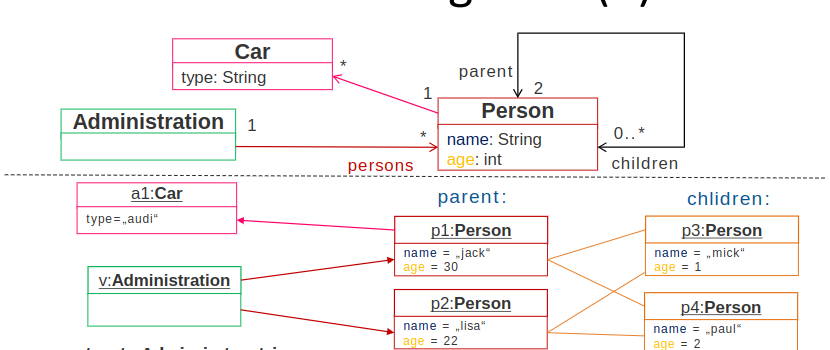
\includegraphics[scale=0.35]{img/exempleNavigation1.png}
\end{wrapfigure}

\noindent\begin{lstlisting}[language=OCL]
  self.persons.children == {p3,p4,p3,p4}
  self.persons.car.type == {"audi"}
\end{lstlisting}

$Self$ représente bien la classe courante d'administration, mais étant donné la multiplicité de la relation $persons$, $self.persons$ représente bien toutes les instances de $Person$ qui font référence à la classe courante d'$Administration$. Il est donc normal que cette expression retourne une collection.

\vspace{0.5cm}

\begin{warningblock}
  Selon la documentation d'OCL, une relation uni-variée ne renverra pas une collection, mais bien la valeur directement.
\end{warningblock}

Dans le cas de relations $0 .. 1$, on peut utiliser l'opération $oclIsUndefined$ afin de vérifier si une valeur existe ou non : 

\begin{lstlisting}[language=OCL]
  context Person inv noChild:
  if self.children.oclIsUndefined() then
    true
  else
    false
  endif
\end{lstlisting}

\subsubsection{Les collections}

Comme vu précédemment, il arrive que l'on récupère des Collections via les relations multivariées, on peut alors utiliser les opérations disponibles par la classe Collection. Mais lorsque l'on utilise une méthode proposée par une Collection, on utilisera l'opérateur $->$. Ainsi, on aura :

\begin{lstlisting}[language=OCL]
  context Person inv noChild2:
    if self.children->isEmpty() then
      true
    else
      false
    endif
\end{lstlisting}

\subsection{Gestion des types}

En OCL, tous les objets sont des sous-types de $OCLAny$. Il fournit les méthodes $oclIsTypeOf$, $oclIsKindOf$ et $oclAsType$

\vspace{0.3cm}

\noindent\textbf{oclIsTypeOf(type : oclType) :} Retourne vrai si l'objet courant est du même type que le paramètre. Il s'agit ici d'avoir exactement le même type, sans prendre en compte les héritages possibles. Pour savoir si deux objets sont du même type au sens de la programmation orientée objet classique, utilisez $oclIsKindOf$.

\subsection{Itération sur les collections}

OCL permet d'itérer sur les collections via des itérateurs prédéfinis.

\subsubsection{Select/Reject}

On peut utiliser les méthodes $select$ et $reject$ pour ne sélectionner que les éléments de la collection qui correspondent ou ne correspondent pas à une condition donnée. Par exemple :

\begin{lstlisting}[language=OCL]
  context Company
  inv QuotaVieux: self.employee->select(age > 50)->notEmpty()
\end{lstlisting}

\subsubsection{Collect}

Similaire à $select$, mais retourne une nouvelle collection sur base de l'existante.

\begin{lstlisting}[language=OCL]
  context Company
  inv OneManOneBirthday : self.employee->collect(birthdate)->asSet()
  -- asSet() means there isn't any duplicate
\end{lstlisting}

\subsubsection{ForAll/Exists}

Vérifie qu'une propriété est respectée par tout/au moins un objet.

\begin{lstlisting}[language=OCL]
  context Company
    inv OneManOneID : self.employees->forAll(e1, e2 | e1 <> e2 implies e1.id <> e2.id)
    inv IWannaSeeTheManager : sef.employees-> exists(e : Employee | e.isManager = true)
\end{lstlisting}

\subsubsection{Itérateur générique}

Manière plus générique d'itérer sur les collections, elle permet de faire toutes les itérations vues précédemment.

\begin{lstlisting}[language=OCL]
  context someContext
    inv SomeInvariant : self.collection->
    iterate(elem: Type, acc : Type = <initExpression> | expression(elem, acc))
\end{lstlisting}

\subsubsection{Closure}

Permet d'itérer récursivement sur une Collection contenant des collections.

\begin{lstlisting}[language=OCL]
  collection ->closure(v : Type | exp(v))
  collection ->closure(v | exp(v))
\end{lstlisting}

\subsection{Opérations sur les objets}

Il y a quelques méthodes mise à disposition par les objets OCL qui peuvent s'avérer pratiques :

\begin{itemize}
  \item \textbf{oclIsNew() : Boolean}
  \begin{itemize}
    \item Retourne vrai si l'objet a été créé durant l'exécution d'opérations juste avant. Cette méthode n'est donc accessible que dans la clause \textit{post}.
  \end{itemize}
  \item \textbf{oclIsInState(t: oclState) : Boolean}
  \begin{itemize}
    \item Retourne vrai si l'objet est dans l'état t.
  \end{itemize}
  \item \textbf{allInstances()}
  \begin{itemize}
    \item Défini sur les classes, les énumérations et les interfaces, retourne toutes les instances d'un type donné.
  \end{itemize}
\end{itemize}

\subsection{Les messages}

Un Observer peut recevoir des messages lors de son exécution. Une fois de plus, cela n'est accessible que dans la clause \textit{post} et on peut s'assurer qu'un message a été reçu :

\begin{lstlisting}[language=OCL]
  context Subject::hasChanged()
    post: observer^update(2,4)
    -- Returns true if an update message was sent with arguments 2 and 4
\end{lstlisting}

On peut aussi récupérer une collection de tous les messages reçus :

\begin{lstlisting}[language=OCL]
  context Subject::hasChanged()
    post: observer^^update(2,4): Sequence(oclMessage)
\end{lstlisting}

\end{document}
